\documentclass[journal,12pt,twocolumn]{IEEEtran}
%
\usepackage{setspace}
\usepackage{gensymb}
\usepackage{xcolor}
\usepackage{caption}
%\usepackage{subcaption}
%\doublespacing
\singlespacing

%\usepackage{graphicx}
%\usepackage{amssymb}
%\usepackage{relsize}
\usepackage[cmex10]{amsmath}
\usepackage{mathtools}
%\usepackage{amsthm}
%\interdisplaylinepenalty=2500
%\savesymbol{iint}
%\usepackage{txfonts}
%\restoresymbol{TXF}{iint}
%\usepackage{wasysym}
\usepackage{hyperref}
\usepackage{amsthm}
\usepackage{mathrsfs}
\usepackage{txfonts}
\usepackage{stfloats}
\usepackage{cite}
\usepackage{cases}
\usepackage{subfig}
%\usepackage{xtab}
\usepackage{longtable}
\usepackage{multirow}
%\usepackage{algorithm}
%\usepackage{algpseudocode}
%\usepackage{enumerate}
\usepackage{enumitem}
\usepackage{mathtools}
%\usepackage{iithtlc}
%\usepackage[framemethod=tikz]{mdframed}
\usepackage{listings}


%\usepackage{stmaryrd}


%\usepackage{wasysym}
%\newcounter{MYtempeqncnt}
\DeclareMathOperator*{\Res}{Res}
%\renewcommand{\baselinestretch}{2}
\renewcommand\thesection{\arabic{section}}
\renewcommand\thesubsection{\thesection.\arabic{subsection}}
\renewcommand\thesubsubsection{\thesubsection.\arabic{subsubsection}}

\renewcommand\thesectiondis{\arabic{section}}
\renewcommand\thesubsectiondis{\thesectiondis.\arabic{subsection}}
\renewcommand\thesubsubsectiondis{\thesubsectiondis.\arabic{subsubsection}}

%\renewcommand{\labelenumi}{\textbf{\theenumi}}
%\renewcommand{\theenumi}{P.\arabic{enumi}}

% correct bad hyphenation here
\hyphenation{op-tical net-works semi-conduc-tor}

\lstset{
language=Python,
frame=single, 
breaklines=true,
columns=fullflexible
}



\begin{document}
%

\theoremstyle{definition}
\newtheorem{theorem}{Theorem}[section]
\newtheorem{problem}{Problem}
\newtheorem{proposition}{Proposition}[section]
\newtheorem{lemma}{Lemma}[section]
\newtheorem{corollary}[theorem]{Corollary}
\newtheorem{example}{Example}[section]
\newtheorem{definition}{Definition}[section]
%\newtheorem{algorithm}{Algorithm}[section]
%\newtheorem{cor}{Corollary}
\newcommand{\BEQA}{\begin{eqnarray}}
\newcommand{\EEQA}{\end{eqnarray}}
\newcommand{\define}{\stackrel{\triangle}{=}}
\bibliographystyle{IEEEtran}
%\bibliographystyle{ieeetr}
\providecommand{\nCr}[2]{\,^{#1}C_{#2}} % nCr
\providecommand{\nPr}[2]{\,^{#1}P_{#2}} % nPr
\providecommand{\mbf}{\mathbf}
\providecommand{\pr}[1]{\ensuremath{\Pr\left(#1\right)}}
\providecommand{\qfunc}[1]{\ensuremath{Q\left(#1\right)}}
\providecommand{\sbrak}[1]{\ensuremath{{}\left[#1\right]}}
\providecommand{\lsbrak}[1]{\ensuremath{{}\left[#1\right.}}
\providecommand{\rsbrak}[1]{\ensuremath{{}\left.#1\right]}}
\providecommand{\brak}[1]{\ensuremath{\left(#1\right)}}
\providecommand{\lbrak}[1]{\ensuremath{\left(#1\right.}}
\providecommand{\rbrak}[1]{\ensuremath{\left.#1\right)}}
\providecommand{\cbrak}[1]{\ensuremath{\left\{#1\right\}}}
\providecommand{\lcbrak}[1]{\ensuremath{\left\{#1\right.}}
\providecommand{\rcbrak}[1]{\ensuremath{\left.#1\right\}}}
\theoremstyle{remark}
\newtheorem{rem}{Remark}
\newcommand{\sgn}{\mathop{\mathrm{sgn}}}
\providecommand{\abs}[1]{\left\vert#1\right\vert}
\providecommand{\res}[1]{\Res\displaylimits_{#1}} 
\providecommand{\norm}[1]{\lVert#1\rVert}
\providecommand{\mtx}[1]{\mathbf{#1}}
\providecommand{\mean}[1]{E\left[ #1 \right]}
\providecommand{\fourier}{\overset{\mathcal{F}}{ \rightleftharpoons}}
\providecommand{\ztrans}{\overset{\mathcal{Z}}{ \rightleftharpoons}}
%\providecommand{\hilbert}{\overset{\mathcal{H}}{ \rightleftharpoons}}
\providecommand{\system}{\overset{\mathcal{H}}{ \longleftrightarrow}}
	%\newcommand{\solution}[2]{\textbf{Solution:}{#1}}
\newcommand{\solution}{\noindent \textbf{Solution: }}
\providecommand{\dec}[2]{\ensuremath{\overset{#1}{\underset{#2}{\gtrless}}}}
\numberwithin{equation}{section}
%\numberwithin{equation}{subsection}
%\numberwithin{problem}{subsection}
%\numberwithin{definition}{subsection}
\makeatletter
\@addtoreset{figure}{problem}
\makeatother
\let\StandardTheFigure\thefigure
%\renewcommand{\thefigure}{\theproblem.\arabic{figure}}
\renewcommand{\thefigure}{\theproblem}
%\numberwithin{figure}{subsection}
\def\putbox#1#2#3{\makebox[0in][l]{\makebox[#1][l]{}\raisebox{\baselineskip}[0in][0in]{\raisebox{#2}[0in][0in]{#3}}}}
     \def\rightbox#1{\makebox[0in][r]{#1}}
     \def\centbox#1{\makebox[0in]{#1}}
     \def\topbox#1{\raisebox{-\baselineskip}[0in][0in]{#1}}
     \def\midbox#1{\raisebox{-0.5\baselineskip}[0in][0in]{#1}}
\vspace{3cm}
\title{ 
%\logo{
Digital Signal Processing
%}
%	\logo{Octave for Math Computing }
}
%\title{
%	\logo{Matrix Analysis through Octave}{\begin{center}\includegraphics[scale=.24]{tlc}\end{center}}{}{HAMDSP}
%}
% paper title
% can use linebreaks \\ within to get better formatting as desired
%\title{Matrix Analysis through Octave}
%
%
% author names and IEEE memberships
% note positions of commas and nonbreaking spaces ( ~ ) LaTeX will not break
% a structure at a ~ so this keeps an author's name from being broken across
% two lines.
% use \thanks{} to gain access to the first footnote area
% a separate \thanks must be used for each paragraph as LaTeX2e's \thanks
% was not built to handle multiple paragraphs
%
\author{ Rohith$^{*}$ %<-this  stops a space
\thanks{*The author is with the Department
of Electrical Engineering, Indian Institute of Technology, Hyderabad
502285 India e-mail:  gadepall@iith.ac.in.  All content in the manuscript is 
released under GNU GPL.  Free to use for anything. }% <-this % stops a space
%\thanks{J. Doe and J. Doe are with Anonymous University.}% <-this % stops a space
%\thanks{Manuscript received April 19, 2005; revised January 11, 2007.}}
}
% note the % following the last \IEEEmembership and also \thanks - 
% these prevent an unwanted space from occurring between the last author name
% and the end of the author line. i.e., if you had this:
% 
% \author{....lastname \thanks{...} \thanks{...} }
%                     ^------------^------------^----Do not want these spaces!
%
% a space would be appended to the last name and could cause every name on that
% line to be shifted left slightly. This is one of those "LaTeX things". For
% instance, "\textbf{A} \textbf{B}" will typeset as "A B" not "AB". To get
% "AB" then you have to do: "\textbf{A}\textbf{B}"
% \thanks is no different in this regard, so shield the last } of each \thanks
% that ends a line with a % and do not let a space in before the next \thanks.
% Spaces after \IEEEmembership other than the last one are OK (and needed) as
% you are supposed to have spaces between the names. For what it is worth,
% this is a minor point as most people would not even notice if the said evil
% space somehow managed to creep in.
% The paper headers
%\markboth{Journal of \LaTeX\ Class Files,~Vol.~6, No.~1, January~2007}%
%{Shell \MakeLowercase{\textit{et al.}}: Bare Demo of IEEEtran.cls for Journals}
% The only time the second header will appear is for the odd numbered pages
% after the title page when using the twoside option.
% 
% *** Note that you probably will NOT want to include the author's ***
% *** name in the headers of peer review papers.                   ***
% You can use \ifCLASSOPTIONpeerreview for conditional compilation here if
% you desire.
% If you want to put a publisher's ID mark on the page you can do it like
% this:
%\IEEEpubid{0000--0000/00\$00.00~\copyright~2007 IEEE}
% Remember, if you use this you must call \IEEEpubidadjcol in the second
% column for its text to clear the IEEEpubid mark.
% make the title area
\maketitle
%\newpage
\tableofcontents
%\renewcommand{\thefigure}{\thesection.\theenumi}
%\renewcommand{\thetable}{\thesection.\theenumi}
\renewcommand{\thefigure}{\theenumi}
\renewcommand{\thetable}{\theenumi}
%\renewcommand{\theequation}{\thesection}
\bigskip
\begin{abstract}
This manual provides a simple introduction to digital signal processing.
\end{abstract}
\section{Software Installation}
Run the following commands
\begin{lstlisting}
sudo apt-get update
sudo apt-get install libffi-dev libsndfile1 python3-scipy  python3-numpy python3-matplotlib 
sudo pip install cffi pysoundfile 
\end{lstlisting}
\section{Digital Filter}
\begin{enumerate}[label=\thesection.\arabic*
,ref=\thesection.\theenumi]
\item
\label{prob:input}
Download the sound file from  
\begin{lstlisting}
wget https://raw.githubusercontent.com/gadepall/ 
EE1310/master/filter/codes/Sound_Noise.wav
\end{lstlisting}
%\href{http://tlc.iith.ac.in/img/sound/Sound_Noise.wav}{\url{http://tlc.iith.ac.in/img/sound/Sound_Noise.wav}}  
%in the link given below.
%\linebreak
\item
\label{prob:spectrogram}
You will find a spectrogram at \href{https://academo.org/demos/spectrum-analyzer}{\url{https://academo.org/demos/spectrum-analyzer}}. 
%\end{problem}
%%
%
%%\onecolumn
%%\input{./figs/fir}
%\begin{problem}
Upload the sound file that you downloaded in Problem \ref{prob:input} in the spectrogram  and play.  Observe the spectrogram. What do you find?
\\
%
\solution There are a lot of yellow lines between 440 Hz to 5.1 KHz.  These represent the synthesizer key tones. Also, the key strokes
are audible along with background noise.
% By observing spectrogram, it clearly shows that tonal frequency is under 4kHz. And above 4kHz only noise is present.
\item
\label{prob:output}
Write the python code for removal of out of band noise and execute the code.
\\
\solution
\lstinputlisting{./codes/2q_cancel_noise.py}
%\begin{figure}[h]
%\centering
%\includegraphics[width=\columnwidth]{enc_block_diag.png}
%\caption{}
%\label{fig:convolution encoder}
%\end{figure}
%\input{block_enc}
\item
The output of the python script in Problem \ref{prob:output} is the audio file Sound\_With\_ReducedNoise.wav. Play the file in the spectrogram in Problem \ref{prob:spectrogram}. What do you observe?
\\
\solution The key strokes as well as background noise is subdued in the audio.  Also,  the signal is blank for frequencies above 5.1 kHz.
\end{enumerate}
\section{Difference Equation}
\begin{enumerate}[label=\thesection.\arabic*,ref=\thesection.\theenumi]
\item Let
	\label{def:xn}
\begin{equation}
x(n) = \cbrak{\underset{\uparrow}{1},2,3,4,2,1}
\end{equation}
Sketch $x(n)$.
\item Let
\begin{multline}
\label{eq:iir_filter}
y(n) + \frac{1}{2}y(n-1) = x(n) + x(n-2), 
\\
 y(n) = 0, n < 0
\end{multline}
Sketch $y(n)$.  
\\
\solution The following code yields Fig. \ref{fig:xnyn}.
\begin{lstlisting}
wget https://github.com/gadepall/EE1310/raw/master/filter/codes/xnyn.py
\end{lstlisting}
\begin{figure}[!ht]
\begin{center}
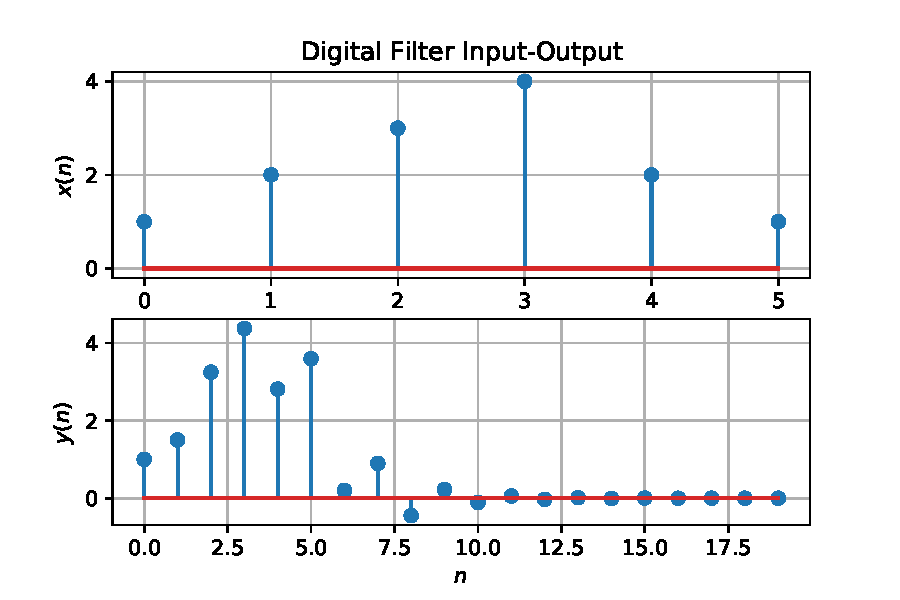
\includegraphics[width=\columnwidth]{./figs/xnyn}
\end{center}
\captionof{figure}{}
\label{fig:xnyn}	
\end{figure}
\item Repeat the above exercise using a C code.
\end{enumerate}
\section{$Z$-transform}
\begin{enumerate}[label=\thesection.\arabic*]
\item The $Z$-transform of $x(n)$ is defined as
%
\begin{equation}
\label{eq:z_trans}
X(z)={\mathcal {Z}}\{x(n)\}=\sum _{n=-\infty }^{\infty }x(n)z^{-n}
\end{equation}
%
Show that
\begin{equation}
\label{eq:shift1}
{\mathcal {Z}}\{x(n-1)\} = z^{-1}X(z)
\end{equation}
and find
\begin{equation}
	{\mathcal {Z}}\{x(n-k)\} 
\end{equation}
\solution From \eqref{eq:z_trans},
\begin{align}
{\mathcal {Z}}\{x(n-k)\} &=\sum _{n=-\infty }^{\infty }x(n-1)z^{-n}
\\
&=\sum _{n=-\infty }^{\infty }x(n)z^{-n-1} = z^{-1}\sum _{n=-\infty }^{\infty }x(n)z^{-n}
\end{align}
resulting in \eqref{eq:shift1}. Similarly, it can be shown that
%
\begin{equation}
\label{eq:z_trans_shift}
	{\mathcal {Z}}\{x(n-k)\} = z^{-k}X(z)
\end{equation}
\item Obtain $X(z)$ for $x(n)$ defined in problem 
	\ref{def:xn}.
\solution 
\begin{equation}
	X(z)=\sum _{n=-\infty }^{\infty }x(n)z^{-n}
	= 1 + \frac{2}{z} +\frac{3}{z^2} + \frac{4}{z^3} + \frac{2}{z^4} + \frac{1}{z^5}
\end{equation}
\item Find
%
\begin{equation}
H(z) = \frac{Y(z)}{X(z)}
\end{equation}
%
from  \eqref{eq:iir_filter} assuming that the $Z$-transform is a linear operation.
\\
\solution  Applying \eqref{eq:z_trans_shift} in \eqref{eq:iir_filter},
\begin{align}
Y(z) + \frac{1}{2}z^{-1}Y(z) &= X(z)+z^{-2}X(z)
\\
\implies \frac{Y(z)}{X(z)} &= \frac{1 + z^{-2}}{1 + \frac{1}{2}z^{-1}}
\label{eq:freq_resp}
\end{align}
%
\item Find the Z transform of 
\begin{equation}
\delta(n)
=
\begin{cases}
1 & n = 0
\\
0 & \text{otherwise}
\end{cases}
\end{equation}
and show that the $Z$-transform of
\begin{equation}
\label{eq:unit_step}
u(n)
=
\begin{cases}
1 & n \ge 0
\\
0 & \text{otherwise}
\end{cases}
\end{equation}
is
\begin{equation}
U(z) = \frac{1}{1-z^{-1}}, \quad \abs{z} > 1
\end{equation}
\solution It is easy to show that
\begin{equation}
\delta(n) \ztrans 1
\end{equation}
and from \eqref{eq:unit_step},
\begin{align}
U(z) &= \sum _{n= 0}^{\infty}z^{-n}
\\
&=\frac{1}{1-z^{-1}}, \quad \abs{z} > 1
\end{align}
using the fomula for the sum of an infinite geometric progression.
%
\item Show that 
\begin{equation}
\label{eq:anun}
a^nu(n) \ztrans \frac{1}{1-az^{-1}} \quad \abs{z} > \abs{a}
\end{equation}
\solution On applying Z-transform:
\begin{align}
	A(z) &= \sum _{n= -{\infty}}^{\infty}a^nu(n)z^{-n}
	\\
	&=\sum _{n= 0}^{\infty}\frac{a^n}{z^{n}}, \quad \abs{z} > \abs{a}
	\\
	&= \frac{1}{1-\frac{a}{z}}
\end{align}
Using the formula for infinite geometric progression with $r = \frac{a}{z}$
\item 
Let
\begin{equation}
H\brak{e^{\j \omega}} = H\brak{z = e^{\j \omega}}.
\end{equation}
Plot $\abs{H\brak{e^{\j \omega}}}$.  Is it periodic? If so, find the period. $H(e^{\j \omega})$ is
known as the {\em Discrete Time Fourier Transform} (DTFT) of $h(n)$.
\\
\solution The following code plots Fig. \ref{fig:dtft}.
\begin{lstlisting}
wget https://raw.githubusercontent.com/gadepall/EE1310/master/filter/codes/dtft.ipynb
\end{lstlisting}
\begin{align}
	H\brak{z} = \frac{1+{z^2}}{{z^2}+{\frac{z}{2}}}
	\\
	H(e^{\j\omega}) = \frac{1+{e^{2\j\omega}}}{{e^{2\j\omega}}+\frac{e^{\j\omega}}{2}}
	\\
	H(e^{\j\omega}) = \frac{2{e^{\j\omega}}\brak{e^{\j\omega}+e^{-{\j\omega}}}}{2e^{2\j\omega}+{e^{\j\omega}}}
	\\
	H(e^{\j\omega}) = \frac{4cos(w)}{1+{2{e^{\j\omega}}}}
	\\
	H\brak{e^{\j \omega}} = \frac{cos(w)}{1+{2cos(w)}+{2jsin(w)}}
	\\
	\abs{H\brak{e^{\j \omega}}} = \frac{\abs{cos(w)}}{\sqrt{5+4cos(w)}}
\end{align}
Therefore, the period is $2{\pi}$
\begin{figure}[!ht]
\centering
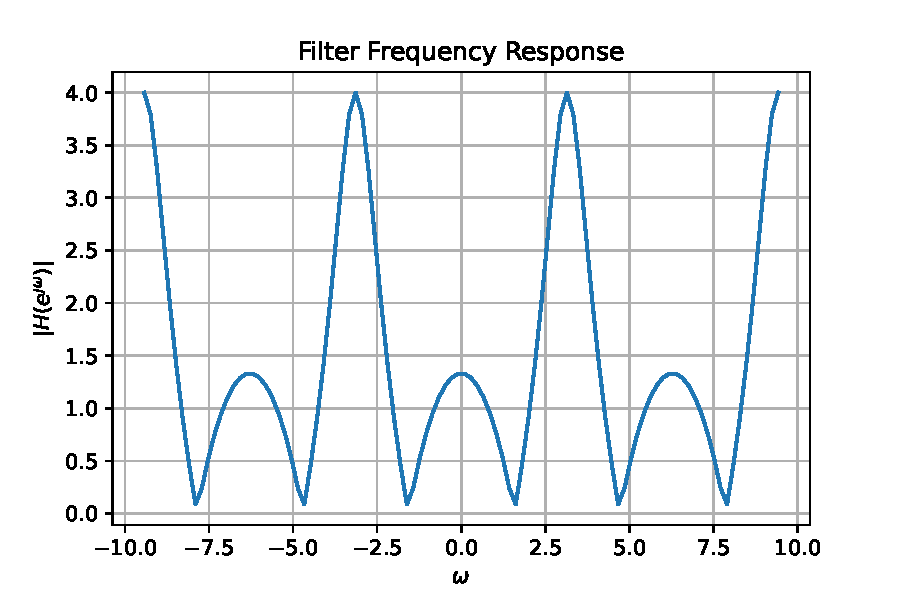
\includegraphics[width=\columnwidth]{./figs/dtft}
\caption{$\abs{H\brak{e^{\j\omega}}}$}
\label{fig:dtft}
\end{figure}
\item Express $h(n)$ in terms of $H\brak{e^{\j \omega}}$.
\end{enumerate}
We know that,
\begin{align}
	H(z) = \sum_{n= -{\infty}}^{\infty}h(n)e^{-\j nz}
\end{align}
Now,
\begin{align}
	\int_{-{\pi}}^{\pi} H(z)e^{\j kz}\, dz\
	\\
	=\int_{-{\pi}}^{\pi} {\sum_{n= -{\infty}}^{\infty}h(n)e^{-\j nz}}e^{\j kz}\, dz\
\end{align}
If n = k, the above integral evaluates to:
\begin{align}
2{\pi}h(k) = 2{\pi}h(n)
\end{align} 
If n ${\neq}$ k, the above integral evaluates to:
\begin{align}
	\sum_{n= -{\infty}}^{\infty}\int_{-{\pi}}^{\pi}h(n)e^{{\j z}(k-n)}\,dz\
	\\
	= \sum_{n= -{\infty}}^{\infty}h(n)\int_{-{\pi}}^{\pi}e^{{\j z}(k-n)}\,dz\
	\\
	= \sum_{n= -{\infty}}^{\infty}h(n)\int_{-{\pi}}^{\pi}cos(z(k-n))+{\j}sin(z(k-n))\,dz\
\end{align}
Taking z(k-n) = t,
\begin{align}
	\sum_{n= -{\infty}}^{\infty}h(n)\int_{-{\pi}(k-n)}^{\pi(k-n)}cos(t)+{\j}sin(t)\,dt\
	\\
	&= 0
\end{align}
\section{Impulse Response}
\begin{enumerate}[label=\thesection.\arabic*]
	\item Using long division, 
find
		\begin{align}
			h(n), \quad n < 5
		\end{align}
		for H(z) in 
		\eqref{eq:freq_resp}.
\\
\solution
\begin{align}
	H(z) = \frac{1+z^{-2}}{1+\frac{z^{-1}}{2}}
\end{align}
Let
\begin{align}
	z^{-1} = t
\end{align}
Hence,
\begin{align}
	1+t^{2} = (2t-4)(1+\frac{t}{2})+5
	\\
	H(z) = (2z^{-1}-4) + \frac{5}{1+\frac{1}{2z}}
	\\
	= \frac{2}{z} - 4 + 5 - \frac{5}{2z} + \frac{5}{4z^{2}}+...
	\\
	= 1 - \frac{1}{2z} + \frac{5}{4z^{2}} - \frac{5}{8z^{3}} + \frac{5}{16z^{4}}
\end{align}
Hence, by comparing with the coefficients with the definition of z-transform
\begin{align}
	h(0) = 1
	\\
	h(1) = -\frac{1}{2}
	\\
	h(2) = \frac{5}{4}
	\\
	h(3) = -\frac{5}{8}
	\\
	h(4) = \frac{5}{16}
\end{align}
\item \label{prob:impulse_resp}
Find an expression for $h(n)$ using $H(z)$, given that 
%in Problem \ref{eq:ztransab} and \eqref{eq:anun}, given that
\begin{equation}
\label{eq:impulse_resp}
h(n) \ztrans H(z)
\end{equation}
and there is a one to one relationship between $h(n)$ and $H(z)$. $h(n)$ is known as the {\em impulse response} of the
system defined by \eqref{eq:iir_filter}.
\\
\solution From \eqref{eq:freq_resp},
\begin{align}
H(z) &= \frac{1}{1 + \frac{1}{2}z^{-1}} + \frac{ z^{-2}}{1 + \frac{1}{2}z^{-1}}
\\
\implies h(n) &= \brak{-\frac{1}{2}}^{n}u(n) + \brak{-\frac{1}{2}}^{n-2}u(n-2)
\end{align}
For $\abs{\frac{1}{2z}}<1$ or $\abs{z}>\frac{1}{2}$
using \eqref{eq:anun} and \eqref{eq:z_trans_shift}.
\item Sketch $h(n)$. Is it bounded? Justify theoretically.
\\
\solution The following code plots Fig. \ref{fig:hn}.
\begin{lstlisting}
wget https://raw.githubusercontent.com/gadepall/EE1310/master/filter/codes/hn.py
\end{lstlisting}
\begin{figure}[!ht]
\centering
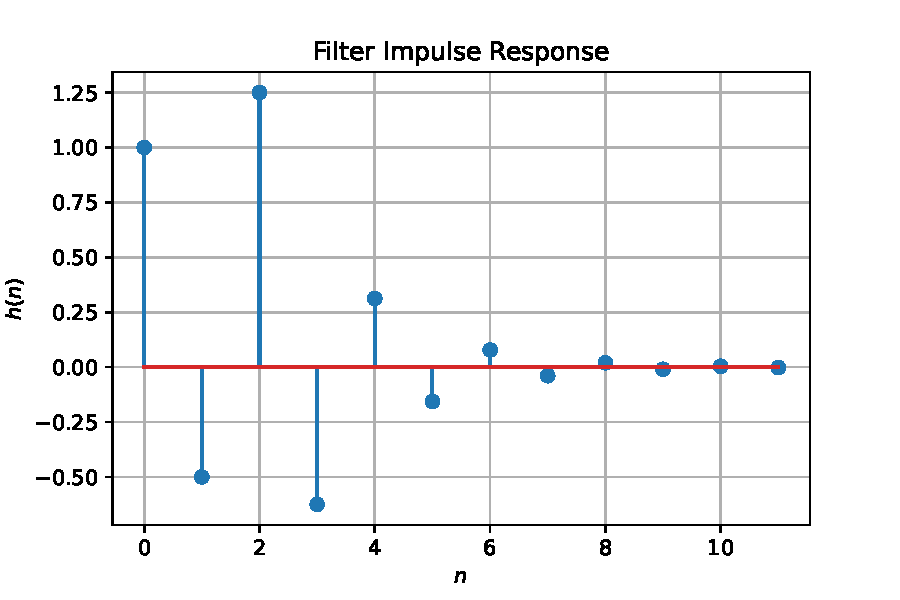
\includegraphics[width=\columnwidth]{./figs/hn}
\caption{$h(n)$ as the inverse of $H(z)$}
\label{fig:hn}
\end{figure}
h(n) is bounded as it tends to 0 as n tends to 12
%
\item Convergent? Justify using the ratio test.
\\
\solution
\begin{align}
	h(n) = (\frac{-1}{2})^{n}u(n) + (\frac{-1}{2})^{n-2}u(n-2)
\end{align}
As n $\to$ $\infty$,
\begin{align}
	h(n)/h(n-1) = \frac{(\frac{-1}{2})^{n} + (\frac{-1}{2})^{n-2}}{(\frac{-1}{2})^{n-1} + (\frac{-1}{2})^{n-3}}
	= -\frac{1}{2}
\end{align}
As $\abs{\frac{h(n)}{h(n-1)}}$$<$1, the series is convergent due to which it is bounded.
\item The system with $h(n)$ is defined to be stable if
\begin{equation}
\sum_{n=-\infty}^{\infty}h(n) < \infty
\end{equation}
Is the system defined by \eqref{eq:iir_filter} stable for the impulse response in \eqref{eq:impulse_resp}?
%
\\
\solution By using h(n) from 5.3
\begin{align}
h(n) &= \brak{-\frac{1}{2}}^{n}u(n) + \brak{-\frac{1}{2}}^{n-2}u(n-2)
\\
&= \sum_{n=-\infty}^{\infty} \brak{-\frac{1}{2}}^{n}u(n) + \brak{-\frac{1}{2}}^{n-2}u(n-2)
\\
&= \sum_{n=-\infty}^{\infty} \brak{-\frac{1}{2}}^{n}u(n) + \sum_{n=-\infty}^{\infty}  \brak{-\frac{1}{2}}^{n-2}u(n-2) 
\\
&= \sum_{n=-\infty}^{\infty} \brak{-\frac{1}{2}}^{n} + \sum_{n=-\infty}^{\infty}  \brak{-\frac{1}{2}}^{n-2}
\\
\\
&= \frac{2}{3} + \frac{2}{3} < \infty 
\end{align}
%
\item Verify the above result using a python code.
\item 
Compute and sketch $h(n)$ using 
\begin{equation}
\label{eq:iir_filter_h}
h(n) + \frac{1}{2}h(n-1) = \delta(n) + \delta(n-2), 
\end{equation}
%
This is the definition of $h(n)$.
\\
\solution The following code plots Fig. \ref{fig:hndef}. Note that this is the same as Fig. 
\ref{fig:hn}. 
%
\begin{lstlisting}
wget https://raw.githubusercontent.com/gadepall/EE1310/master/filter/codes/hndef.ipynb
\end{lstlisting}
\begin{figure}[!ht]
\centering
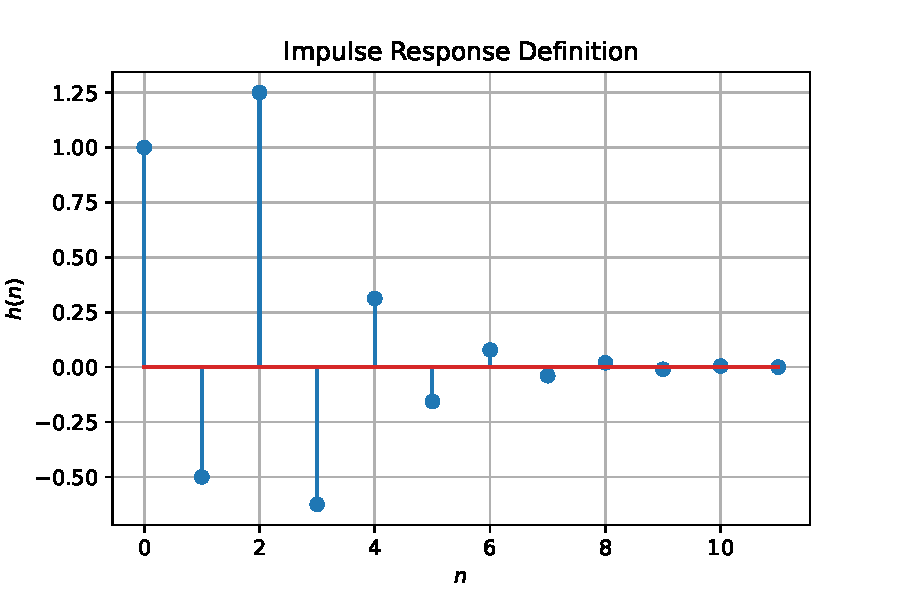
\includegraphics[width=\columnwidth]{./figs/hndef}
\caption{$h(n)$ from the definition}
\label{fig:hndef}
\end{figure}
%
\item Compute 
%
\begin{equation}
\label{eq:convolution}
y(n) = x(n)*h(n) = \sum_{n=-\infty}^{\infty}x(k)h(n-k)
\end{equation}
%
Comment. The operation in \eqref{eq:convolution} is known as
{\em convolution}.
%
\\
\solution The following code plots Fig. \ref{fig:ynconv}. Note that this is the same as 
$y(n)$ in  Fig. 
\ref{fig:xnyn}. 
%
\begin{lstlisting}
wget https://raw.githubusercontent.com/gadepall/EE1310/master/filter/codes/ynconv.ipynb
\end{lstlisting}
\begin{figure}[!ht]
\centering
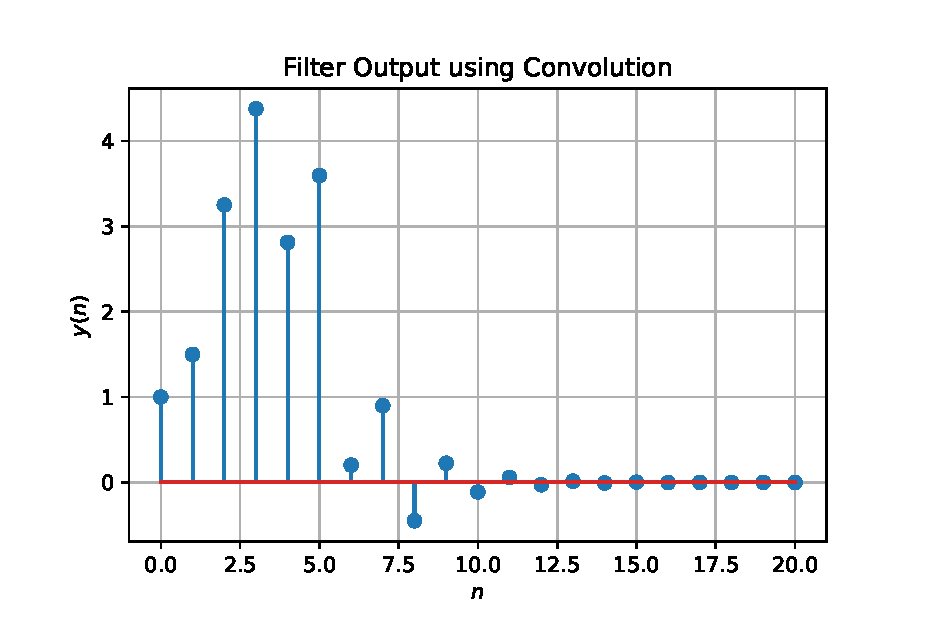
\includegraphics[width=\columnwidth]{./figs/ynconv}
\caption{$y(n)$ from the definition of convolution}
\label{fig:ynconv}
\end{figure}
\item Express the above convolution using a Teoplitz matrix.
\item Show that
\begin{equation}
y(n) =  \sum_{n=-\infty}^{\infty}x(n-k)h(k)
\end{equation}
\solution
We know that,
\begin{align}
	y(n) = \sum_{n=-\infty}^{\infty}x(k)h(n-k)
\end{align}
Taking k = n-k
\begin{align}
	y(n) =  \sum_{n=-\infty}^{\infty}x(n-k)h(k)
\end{align}
\item Oppenheimer question 
\begin{align}
	x[n] = u[n+10]-u[n+5]
	\\
	=
	\begin{cases}
		1 & -10<=n<-6
		\\	
		0 & otherwise
	\end{cases}
\end{align}
x[n] is finite length and has only positive powers of z, hence, its ROC is $\abs{z}<\infty$
\end{enumerate}
%
\section{DFT}
\begin{enumerate}[label=\thesection.\arabic*]
\item
Compute
\begin{equation}
X(k) \define \sum _{n=0}^{N-1}x(n) e^{-\j2\pi kn/N}, \quad k = 0,1,\dots, N-1
\end{equation}
and $H(k)$ using $h(n)$.
\item Compute 
\begin{equation}
Y(k) = X(k)H(k)
\end{equation}
\item Compute
\begin{equation}
 y\brak{n}={\frac {1}{N}}\sum _{k=0}^{N-1}Y\brak{k}\cdot e^{\j 2\pi kn/N},\quad n = 0,1,\dots, N-1
\end{equation}
\\
\solution The following code plots Fig. \ref{fig:ynconv}. Note that this is the same as 
$y(n)$ in  Fig. 
\ref{fig:xnyn}. 
%
\begin{lstlisting}
wget https://raw.githubusercontent.com/gadepall/EE1310/master/filter/codes/yndft.ipynb
\end{lstlisting}
\begin{figure}[!ht]
\centering
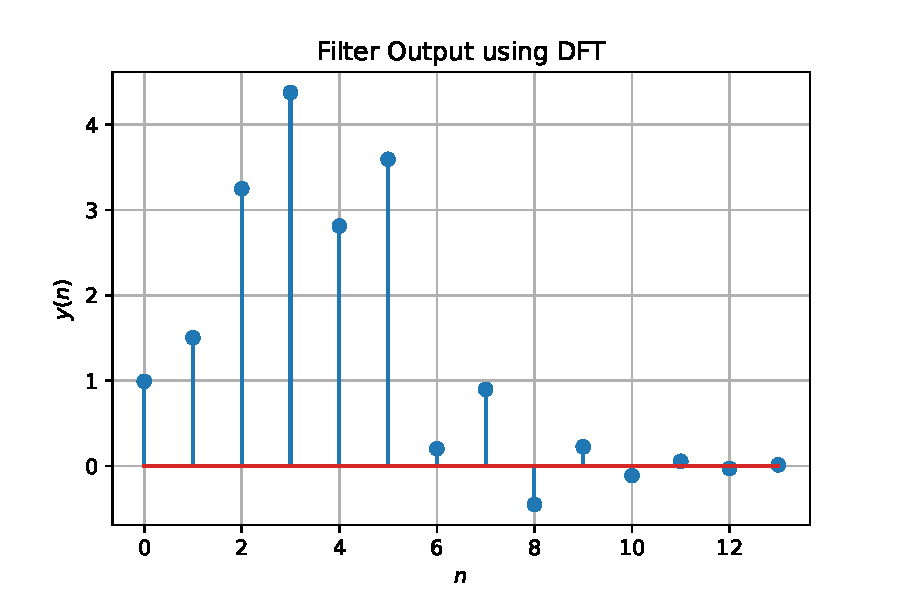
\includegraphics[width=\columnwidth]{./figs/yndft}
\caption{$y(n)$ from the DFT}
\label{fig:yndft}
\end{figure}
\item Repeat the previous exercise by computing $X(k), H(k)$ and $y(n)$ through FFT and 
IFFT.
\end{enumerate}
%
\section{FFT}
% \subsection{Definitions}
\begin{enumerate}[label=\arabic*.,ref=\thesection.\theenumi]
\numberwithin{equation}{section}
    \item The DFT of $x(n)$ is given by
    \begin{align}
        X(k) \triangleq \sum_{n=0}^{N-1} x(n) e^{-j 2 \pi k n / N}, \quad k=0,1, \ldots, N-1
    \end{align}
\item Let 
	\begin{align}
W_{N} = e^{-j2\pi/N} 
	\end{align}
		Then the $N$-point {\em DFT matrix} is defined as 
	\begin{align}
		\vec{F}_{N} = \sbrak{W_{N}^{mn}}, \quad 0 \le m,n \le N-1 
	\end{align}
	where $W_{N}^{mn}$ are the elements of $\vec{F}_{N}$.
\item Let 
	\begin{align}
		\vec{I}_4 = \myvec{\vec{e}_4^{1} &\vec{e}_4^{2} &\vec{e}_4^{3} &\vec{e}_4^{4} }
	\end{align}
		be the $4\times 4$ identity matrix.  Then the 4 point {\em DFT permutation matrix} is defined as 
	\begin{align}
		\vec{P}_4 = \myvec{\vec{e}_4^{1} &\vec{e}_4^{3} &\vec{e}_4^{2} &\vec{e}_4^{4} }
	\end{align}
\item The 4 point {\em DFT diagonal matrix} is defined as 
	\begin{align}
		\vec{D}_4 = diag\myvec{W_{8}^{0} & W_{8}^{1} & W_{8}^{2} & W_{8}^{3}}
	\end{align}
\item Show that 
\begin{equation}
    W_{N}^{2}=W_{N/2}
\end{equation}
\begin{solution}
	\begin{align}
		W_{N}^{2} = {e}^{-j*2*2\pi/N}
		\\
		= {e}^{-j2\pi/(N/2)}
		\\
		= W_{N/2}
	\end{align}
\end{solution}
%    \item Find $\vec{P}_6$.
%    \item Find $\vec{D}_3$.
    \item Show that 
\begin{equation}
	\vec{F}_{4}=
\begin{bmatrix}
	\vec{I}_{2} & \vec{D}_{2} \\
\vec{I}_{2} & -\vec{D}_{2}
\end{bmatrix}
\begin{bmatrix}
\vec{F}_{2} & 0 \\
0 & \vec{F}_{2}
\end{bmatrix}
\vec{P}_{4}
\end{equation}
\begin{solution}
	\begin{equation}
	\vec{F}_{4}=
	\begin{bmatrix}
		1 & 1 & 1 & 1 \\
		1 & \vec{W_{N}} & \vec{W_{N}^{2}} & \vec{W_{N}^{3}}\\
		1 & \vec{W_{N}^{2}} & \vec{W_{N}^{4}} & \vec{W_{N}^{6}}\\
		1 & \vec{W_{N}^{3}} & \vec{W_{N}^{6}} & \vec{W_{N}^{9}}
	\end{bmatrix}
\end{equation}
On post multiplying $F_{4}$ with $P_{4}$  and using $W_{N}^{4} = 1$ we get,
\begin{equation}
	\vec{F}_{4}\vec{P}_{4}=
	\begin{bmatrix}
		1 & 1 & 1 & 1 \\
		1 & \vec{W_{N}^2} & \vec{W_{N}} & \vec{W_{N}^{3}}\\
		1 & 1 & \vec{W_{N}^{2}} & \vec{W_{N}^{6}}\\
		1 & \vec{W_{N}^{2}} & \vec{W_{N}^{3}} & \vec{W_{N}^{9}}
	\end{bmatrix}
\end{equation}
Using $W_{N}^{2} = W_{N/2}$, upper left and lower left $2*2$ matrices
become equal to $F_{2}$. The top right matrix =
\begin{equation}
	\begin{bmatrix}
		1 & 1 \\
		\vec{W_{N}} & \vec{W_{N}^{3}}
	\end{bmatrix}
\end{equation}
=
\begin{equation}
	\begin{bmatrix}
		1 & 0 \\
		0 & \vec{W_{N}}
	\end{bmatrix}
	\begin{bmatrix}
		1 & 1 \\
		1 & \vec{W_{N}^{2}}
	\end{bmatrix}
\end{equation}
= ${D_{2}}{F_{2}}$
\\
Similarly, bottom right matrix = 
= -${D_{2}}{F_{2}}$
\\
Hence,
\\${F_{4}{P_{4}}}$ = 
\begin{equation}
	\begin{bmatrix}
		\vec{F_{2}} & \vec{D_{2}F_{2}} \\
		\vec{F_{2}} & -\vec{D_{2}F_{2}}
	\end{bmatrix}
\end{equation}
\\=
\begin{equation}
\begin{bmatrix}
	\vec{I}_{2} & \vec{D}_{2} \\
\vec{I}_{2} & -\vec{D}_{2}
\end{bmatrix}
\begin{bmatrix}
\vec{F}_{2} & 0 \\
0 & \vec{F}_{2}
\end{bmatrix}
\end{equation}
\end{solution}
\item Show that 
\begin{equation}
\vec{F}_{N}=
\begin{bmatrix}
\vec{I}_{N/2} & \vec{D}_{N/2} \\
\vec{I}_{N/2} & -\vec{D}_{N/2}
\end{bmatrix}
\begin{bmatrix}
\vec{F}_{N/2} & 0 \\
0 & \vec{F}_{N/2}
\end{bmatrix}
\vec{P}_{N}
\end{equation}
\begin{solution}
	Similar to the above, we post multiply $F_{N}$ with $P_{N}$
	so that the resultant matrix can be split into 4 parts:
	top-left, top-right, bottom-left and bottom-right: all being 
	${n/2}*{n/2}$ square matrices.
	\\
	Top left matrix = Bottom left matrix = $F_{N/2}$
	\\
	Top right matrix = $D_{N/2}$$F_{N/2}$
	\\
	Bottom right matrix = -$D_{N/2}$$F_{N/2}$
	Hence,
\\${F_{N}{P_{N}}}$ = 
\begin{equation}
	\begin{bmatrix}
		\vec{F_{N/2}} & \vec{D_{N/2}F_{N/2}} \\
		\vec{F_{N/2}} & -\vec{D_{N/2}F_{N/2}}
	\end{bmatrix}
\end{equation}
\end{solution}
\item Find 
    \begin{align}
	     \vec{P}_4 \vec{x}
    \end{align}
\begin{solution}
	\\
	$\vec{x}$ =
	\\
\begin{equation}
	\begin{bmatrix}
		1 \\
		2 \\
		3 \\
		4 \\
		2 \\
		1 \\
	\end{bmatrix}
\end{equation}
So, $\vec{P_{4}}\vec{x}$ = 
\begin{equation}
	\begin{bmatrix}
		1 \\
		3 \\
		2 \\
		4 \\
		0 \\
		0 \\
	\end{bmatrix}
\end{equation}
\end{solution}
\item Show that 
    \begin{align}
	    \vec{X} = \vec{F}_N \vec{x}
	    \label{eq:dft-mat-def}
    \end{align}
		where $\vec{x}, \vec{X}$ are the vector representations of $x(n), X(k)$ respectively.\
\\		
\begin{solution}
\\
$\vec{x}$ =
\begin{equation}
	\begin{bmatrix}
		x[0] \\
		x[1] \\
		x[2] \\
		. \\
		. \\
		. \\
		x[n-1]
	\end{bmatrix}
\end{equation}
$F_{N}$ =
\\
\begin{equation}
	\begin{bmatrix}
		1 & 1 & 1 & . & . & . 1 \\
		1 & W_N & W_N^{2} & . & . &. W_N^{N-1}\\
		1 & W_N^{2} & W_N^{4} & . & . &. W_N^{2N-2} \\
		. & . & . & . & . &. W_N^{3N-3}\\
		. \\
		. \\
		1 & W_N^{N-1} & W_N^{2(N-1)} & . & . &. W_N^{N(N-1)}
	\end{bmatrix}
\end{equation}
\\
$\vec{X}$ =
\begin{equation}
	\begin{bmatrix}
		X[0] \\
		X[1] \\
		X[2] \\
		. \\
		. \\
		. \\
		X[n-1]
	\end{bmatrix}
\end{equation}
By definition, $X[k]$ = $\sum_{n=0}^{N-1}x(n)e^{-2*\pi*j*k*n}$
\\Hence, by the definition of matrix multiplication:
\\$\vec{X} = \vec{F_{N}}\vec{x}$ =
\begin{equation}
	\begin{bmatrix}
		1 & 1 & 1 & . & . & . 1 \\
		1 & W_N & W_N^{2} & . & . &. W_N^{N-1}\\
		1 & W_N^{2} & W_N^{4} & . & . &. W_N^{2N-2} \\
		. & . & . & . & . &. W_N^{3N-3}\\
		. \\
		. \\
		1 & W_N^{N-1} & W_N^{2(N-1)} & . & . &. W_N^{N(N-1)}
	\end{bmatrix}
	\begin{bmatrix}
		x[0] \\
		x[1] \\
		x[2] \\
		. \\
		. \\
		. \\
		x[N-1]
	\end{bmatrix}
\end{equation}
\end{solution}
\item Derive the following Step-by-step visualisation  of
8-point FFTs into 4-point FFTs and so on
\begin{equation}
\begin{bmatrix}
X(0) \\ 
X(1) \\ 
X(2) \\ 
X(3)
\end{bmatrix}
=
\begin{bmatrix}
X_{1}(0) \\ 
X_{1}(1)\\ 
X_{1}(2)\\
X_{1}(3)\\
\end{bmatrix}
+
\begin{bmatrix}
W^{0}_{8} & 0 & 0 & 0\\
0 & W^{1}_{8} & 0 & 0\\
0 & 0 & W^{2}_{8} & 0\\
0 & 0 & 0 & W^{3}_{8}
\end{bmatrix}
\begin{bmatrix}
X_{2}(0) \\ 
X_{2}(1) \\ 
X_{2}(2) \\
X_{2}(3)
\end{bmatrix}
\end{equation}
\begin{equation}
\begin{bmatrix}
X(4) \\ 
X(5) \\ 
X(6) \\ 
X(7)
\end{bmatrix}
=
\begin{bmatrix}
X_{1}(0) \\ 
X_{1}(1)\\ 
X_{1}(2)\\
X_{1}(3)\\
\end{bmatrix}
-
\begin{bmatrix}
W^{0}_{8} & 0 & 0 & 0\\
0 & W^{1}_{8} & 0 & 0\\
0 & 0 & W^{2}_{8} & 0\\
0 & 0 & 0 & W^{3}_{8}
\end{bmatrix}
\begin{bmatrix}
X_{2}(0) \\ 
X_{2}(1) \\ 
X_{2}(2) \\
X_{2}(3)
\end{bmatrix}
\end{equation}
4-point FFTs into 2-point FFTs
\begin{equation}
\begin{bmatrix}
X_{1}(0) \\ 
X_{1}(1)\\ 
\end{bmatrix}
=
\begin{bmatrix}
X_{3}(0) \\ 
X_{3}(1)\\ 
\end{bmatrix}
+
\begin{bmatrix}
W^{0}_{4} & 0\\
0 & W^{1}_{4}
\end{bmatrix}
\begin{bmatrix}
X_{4}(0) \\ 
X_{4}(1) \\ 
\end{bmatrix}
\end{equation}
\begin{equation}
\begin{bmatrix}
X_{1}(2) \\ 
X_{1}(3)\\ 
\end{bmatrix}
=
\begin{bmatrix}
X_{3}(0) \\ 
X_{3}(1)\\ 
\end{bmatrix}
-
\begin{bmatrix}
W^{0}_{4} & 0\\
0 & W^{1}_{4}
\end{bmatrix}
\begin{bmatrix}
X_{4}(0) \\ 
X_{4}(1) \\ 
\end{bmatrix}
\end{equation}
\begin{equation}
\begin{bmatrix}
X_{2}(0) \\ 
X_{2}(1)\\ 
\end{bmatrix}
=
\begin{bmatrix}
X_{5}(0) \\ 
X_{5}(1)\\ 
\end{bmatrix}
+
\begin{bmatrix}
W^{0}_{4} & 0\\
0 & W^{1}_{4}
\end{bmatrix}
\begin{bmatrix}
X_{6}(0) \\ 
X_{6}(1) \\ 
\end{bmatrix}
\end{equation}
\begin{equation}
\begin{bmatrix}
X_{2}(2) \\ 
X_{2}(3)\\ 
\end{bmatrix}
=
\begin{bmatrix}
X_{5}(0) \\ 
X_{5}(1)\\ 
\end{bmatrix}
-
\begin{bmatrix}
W^{0}_{4} & 0\\
0 & W^{1}_{4}
\end{bmatrix}
\begin{bmatrix}
X_{6}(0) \\ 
X_{6}(1) \\ 
\end{bmatrix}
\end{equation}
\begin{equation}
P_{8}
\begin{bmatrix}
x(0) \\ 
x(1) \\ 
x(2) \\ 
x(3) \\ 
x(4) \\ 
x(5) \\
x(6) \\
x(7)
\end{bmatrix}
 = 
\begin{bmatrix}
x(0) \\ 
x(2) \\ 
x(4) \\ 
x(6) \\
x(1) \\ 
x(3) \\ 
x(5) \\
x(7)
\end{bmatrix}
\end{equation}
\begin{equation}
P_{4}
\begin{bmatrix}
x(0) \\ 
x(2) \\ 
x(4) \\ 
x(6) \\
\end{bmatrix}
 = 
\begin{bmatrix}
x(0) \\ 
x(4) \\ 
x(2) \\
x(6)
\end{bmatrix}
\end{equation}
\begin{equation}
P_{4}
\begin{bmatrix}
x(1) \\ 
x(3) \\ 
x(5) \\
x(7)
\end{bmatrix}
 = 
\begin{bmatrix}
x(1) \\ 
x(5) \\ 
x(3) \\ 
x(7) \\
\end{bmatrix}
\end{equation}
Therefore,
\begin{equation}
\begin{bmatrix}
X_{3}(0) \\ 
X_{3}(1)\\ 
\end{bmatrix}
= F_{2}
\begin{bmatrix}
x(0) \\ 
x(4) \\ 
\end{bmatrix}
\end{equation}
\begin{equation}
\begin{bmatrix}
X_{4}(0) \\ 
X_{4}(1)\\ 
\end{bmatrix}
= F_{2}
\begin{bmatrix}
x(2) \\ 
x(6) \\ 
\end{bmatrix}
\end{equation}
\begin{equation}
\begin{bmatrix}
X_{5}(0) \\ 
X_{5}(1)\\ 
\end{bmatrix}
= F_{2}
\begin{bmatrix}
x(1) \\ 
x(5) \\ 
\end{bmatrix}
\end{equation}
\begin{equation}
\begin{bmatrix}
X_{6}(0) \\ 
X_{6}(1)\\ 
\end{bmatrix}
= F_{2}
\begin{bmatrix}
x(3) \\ 
x(7) \\ 
\end{bmatrix}
\end{equation}
\begin{solution}
\\
For every k, X[k] = 
\begin{equation}
	\\
	\sum_{0}^{7}x(n)e^{-2jkn\pi/8}
	\\
	= \sum_{0}^{3}x(2n)e^{-2jk(2n)\pi/8}+\sum_{0}^{3}x(2n+1)e^{-2jk(2n+1)\pi/8}
\end{equation}
\\=
\begin{equation}
	\\
	= \sum_{0}^{3}x(2n)e^{-2jk(n)\pi/4}+e^{-2kj\pi/8}(\sum_{0}^{3}x(2n+1)e^{-2jk(n)\pi/4})
\end{equation}
\\=
$X_1$[k]+$e^{-2kj\pi/8}$$X_2[k]$, where $X_1$[k] is FFT of even terms
and $X_2$[k] is FFT of odd terms.
\\
Also, if k$>=$4,
\\
$e^{-2jk\pi/8}$ = -$e^{-2j(k-4)\pi/8}$ 
\\Hence,
\begin{equation}
\begin{bmatrix}
	X(0) \\ 
	X(1) \\
	X(2) \\
	X(3) \\
\end{bmatrix}
=
\begin{bmatrix}
	X_1(0) \\ 
	X_1(1) \\
	X_1(2) \\
	X_1(3) \\
\end{bmatrix}
+
\begin{bmatrix}
	W_8^{0} & 0 & 0 & 0\\ 
	0 & W_8^{1} & 0 & 0 \\
	0 & 0 & W_8^{2} & 0 \\
	0 & 0 & 0 & W_8^{3} \\
\end{bmatrix}
\begin{bmatrix}
	X_2(0) \\ 
	X_2(1) \\
	X_2(2) \\
	X_2(3) \\
\end{bmatrix}
\end{equation}
\begin{equation}
\begin{bmatrix}
	X(4) \\ 
	X(5) \\
	X(6) \\
	X(7) \\
\end{bmatrix}
=
\begin{bmatrix}
	X_1(0) \\ 
	X_1(1) \\
	X_1(2) \\
	X_1(3) \\
\end{bmatrix}
-
\begin{bmatrix}
	W_8^{0} & 0 & 0 & 0\\ 
	0 & W_8^{1} & 0 & 0 \\
	0 & 0 & W_8^{2} & 0 \\
	0 & 0 & 0 & W_8^{3} \\
\end{bmatrix}
\begin{bmatrix}
	X_2(0) \\ 
	X_2(1) \\
	X_2(2) \\
	X_2(3) \\
\end{bmatrix}
\end{equation}
Decomposing into 2 point dft matrices:
\begin{equation}
	\begin{bmatrix}
	X_{1}(0) \\ 
	X_{1}(1)\\ 
	\end{bmatrix}
	=
	\begin{bmatrix}
	X_{3}(0) \\ 
	X_{3}(1)\\ 
	\end{bmatrix}
	+
	\begin{bmatrix}
	W^{0}_{4} & 0\\
	0 & W^{1}_{4}
	\end{bmatrix}
	\begin{bmatrix}
	X_{4}(0) \\ 
	X_{4}(1) \\ 
	\end{bmatrix}
	\end{equation}
	\begin{equation}
	\begin{bmatrix}
	X_{1}(2) \\ 
	X_{1}(3)\\ 
	\end{bmatrix}
	=
	\begin{bmatrix}
	X_{3}(0) \\ 
	X_{3}(1)\\ 
	\end{bmatrix}
	-
	\begin{bmatrix}
	W^{0}_{4} & 0\\
	0 & W^{1}_{4}
	\end{bmatrix}
	\begin{bmatrix}
	X_{4}(0) \\ 
	X_{4}(1) \\ 
	\end{bmatrix}
	\end{equation}
	\begin{equation}
	\begin{bmatrix}
	X_{2}(0) \\ 
	X_{2}(1)\\ 
	\end{bmatrix}
	=
	\begin{bmatrix}
	X_{5}(0) \\ 
	X_{5}(1)\\ 
	\end{bmatrix}
	+
	\begin{bmatrix}
	W^{0}_{4} & 0\\
	0 & W^{1}_{4}
	\end{bmatrix}
	\begin{bmatrix}
	X_{6}(0) \\ 
	X_{6}(1) \\ 
	\end{bmatrix}
	\end{equation}
	\begin{equation}
	\begin{bmatrix}
	X_{2}(2) \\ 
	X_{2}(3)\\ 
	\end{bmatrix}
	=
	\begin{bmatrix}
	X_{5}(0) \\ 
	X_{5}(1)\\ 
	\end{bmatrix}
	-
	\begin{bmatrix}
	W^{0}_{4} & 0\\
	0 & W^{1}_{4}
	\end{bmatrix}
	\begin{bmatrix}
	X_{6}(0) \\ 
	X_{6}(1) \\ 
	\end{bmatrix}
	\end{equation}
\end{solution}
\item For 
    \begin{align}
	    \vec{x} = \myvec{1\\2\\3\\4\\2\\1}
        \label{eq:equation1}
    \end{align}
    compte the DFT  
		using 
	    \eqref{eq:dft-mat-def}
\\
\begin{solution}
	\\$\vec{F_6}$ = $\begin{bmatrix}W_6^{MN}\end{bmatrix}$
	\\Where M is the index of row of matrix and N the index of column of matrix
	\\$\vec{F_6}\vec{x}$
	\\ =
	\begin{equation}
		\begin{bmatrix}
			13 \\
			-4-\sqrt{3}j \\
			1 \\
			-1 \\
			1 \\
			-4 + \sqrt{3}j \\
		\end{bmatrix}
	\end{equation}
\end{solution}
    \item Repeat the above exercise using the FFT
	    after zero padding $\vec{x}$.
%	    \eqref{eq:fft-mat-def}
\\
\begin{solution}
	\\$\vec{x}$ = 
	\begin{equation}
		\begin{bmatrix}
			1 \\
			2 \\
			3 \\
			4 \\
			2 \\
			1 \\
			0 \\
			0 \\
		\end{bmatrix}
	\end{equation}
	\\
	Using ,
	\begin{align}
	\vec{F}_{8}=
	\begin{bmatrix}
	\vec{I}_{4} & \vec{D}_{4} \\
	\vec{I}_{4} & -\vec{D}_{4}
	\end{bmatrix}
	\begin{bmatrix}
	\vec{F}_{4} & 0 \\
	0 & \vec{F}_{4}
	\end{bmatrix}
	\vec{P}_{8}\\
	\vec{F}_{4}=
	\begin{bmatrix}
	\vec{I}_{2} & \vec{D}_{2} \\
	\vec{I}_{2} & -\vec{D}_{2}
	\end{bmatrix}
	\begin{bmatrix}
	\vec{F}_{2} & 0 \\
	0 & \vec{F}_{2}
	\end{bmatrix}
	\vec{P}_{4}\\
	\vec{F}_{2}=
	\begin{bmatrix}
	\vec{I}_{1} & \vec{D}_{1} \\
	\vec{I}_{1} & -\vec{D}_{1}
	\end{bmatrix}
	\begin{bmatrix}
	\vec{F}_{1} & 0 \\
	0 & \vec{F}_{1}
	\end{bmatrix}
	\vec{P}_{2}\\
	\vec{F_1}=\sbrak{1}
	\end{align}
	Calculating $\vec{F_2}$,
\begin{align}
\vec{F_2}&=\begin{bmatrix}
\vec{F}_{1} & \vec{D_1F_1} \\
\vec{F}_{1} & -\vec{D_1F_1}
\end{bmatrix}\vec{P_2}\\
&=\begin{bmatrix}1&1\\1&-1\end{bmatrix}
\end{align}
Calculating $\vec{F_4}$,
\begin{align}
\vec{D}_{2}=diag(1,W_4)
=\begin{bmatrix}
1&0\\0&-j
\end{bmatrix}\\
\vec{D_2F_2}=\begin{bmatrix}
1&0\\0&-j
\end{bmatrix}\begin{bmatrix}
1&1\\1&-1
\end{bmatrix}\\
=\begin{bmatrix}
1&1\\-j&j
\end{bmatrix}\\
\vec{F_4}=\begin{bmatrix}
\vec{F}_{2} & \vec{D_2F_2} \\
\vec{F}_{2} & -\vec{D_2F_2}
\end{bmatrix}\vec{P_4}\\
\vec{F_4}=\begin{bmatrix}
1&0&1&1\\0&1&-j&j\\1&0&-1&-1\\0&1&j&-j
\end{bmatrix}\begin{bmatrix}
1&0&0&0\\0&0&1&0\\0&1&0&0\\0&0&0&1
\end{bmatrix}\\
=\begin{bmatrix}
1&1&0&1\\0&-j&1&j\\1&-1&0&j\\0&j&1&-j
\end{bmatrix}
\end{align}
Calculating $\vec{F_8}$,
\begin{align}
\vec{D_4}=diag\brak{1,W_8,W_8^2,W_8^3}\\
=\begin{bmatrix}
1&0&0&0\\0&\frac{1-j}{\sqrt{2}}&0&0\\0&0&-1&0\\0&0&0&\frac{-1-j}{\sqrt{2}}
\end{bmatrix}\\
\vec{D_4F_4}=\begin{bmatrix}
1&0&0&0\\0&\frac{1-j}{\sqrt{2}}&0&0\\0&0&-1&0\\0&0&0&\frac{-1-j}{\sqrt{2}}
\end{bmatrix}\begin{bmatrix}
1&1&0&1\\0&-j&1&j\\1&-1&0&j\\0&j&1&-j
\end{bmatrix}\\
=\begin{bmatrix}
1&1&0&1\\0&\frac{-1-j}{\sqrt{2}}&\frac{1-j}{\sqrt{2}}&\frac{1+j}{\sqrt{2}}\\-1&1&0&-j\\0&\frac{1-j}{\sqrt{2}}&\frac{-1-j}{\sqrt{2}}&\frac{-1+j}{\sqrt{2}}
\end{bmatrix}
\end{align}
Therefore, from $F_8$,
\begin{align}
\vec{X}=\begin{bmatrix}
	 13\\-3.12-6.53j\\j\\1.12-0.53j\\-1\\1.12+0.53j\\-j\\-3.12+6.5355
	 \end{bmatrix}
\end{align}
\end{solution}
\graphicspath{ {./figs/} }
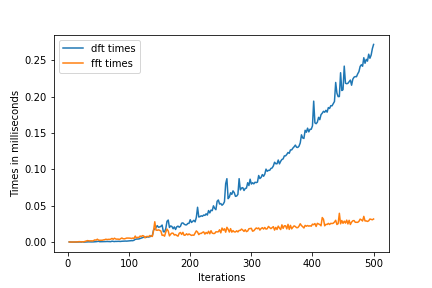
\includegraphics[scale=0.5]{dft_fft_times.png}
\item Write a C program to compute the 8-point FFT.
\begin{solution}
	\lstinputlisting{./codes/fft.c}
\end{solution} 
 \end{enumerate}

\end{document}